\documentclass[11pt,a4paper]{article}

% ============ PACKAGES ============
\usepackage[utf8]{inputenc}
\usepackage[T1]{fontenc}
\usepackage[margin=1in]{geometry}
\sloppy
\usepackage{amsmath,amssymb,amsthm}
\usepackage{booktabs}
\usepackage{array}
\usepackage{enumitem}
\usepackage{fancyhdr}
\usepackage{hyperref}
\usepackage{xcolor}
\usepackage{tcolorbox}
\tcbuselibrary{breakable}
\usepackage{float}
\usepackage{listings}
\usepackage{tikz}
\usetikzlibrary{shapes.geometric, arrows.meta, positioning, fit}

% ============ COLORS ============
\definecolor{codeblue}{rgb}{0.13,0.29,0.53}
\definecolor{passgreen}{rgb}{0,0.5,0}
\definecolor{failred}{rgb}{0.8,0,0}
\definecolor{codegray}{rgb}{0.5,0.5,0.5}
\definecolor{backcolour}{rgb}{0.97,0.97,0.97}
\definecolor{notebg}{rgb}{0.93,0.95,1.0}
\definecolor{noteborder}{rgb}{0.4,0.5,0.7}
\definecolor{warningbg}{rgb}{1.0,0.97,0.88}
\definecolor{warningborder}{rgb}{1.0,0.6,0.0}
\definecolor{scenariobg}{rgb}{0.95,1.0,0.95}
\definecolor{scenarioborder}{rgb}{0.2,0.6,0.3}
\definecolor{criticalbg}{rgb}{1.0,0.92,0.92}
\definecolor{criticalborder}{rgb}{0.8,0.2,0.2}

% ============ THEOREM ENVIRONMENTS ============
\theoremstyle{definition}
\newtheorem{definition}{Definition}[section]
\newtheorem{invariant}{Invariant}[section]

% ============ BOXES ============
\newtcolorbox{notebox}{
    colback=notebg, colframe=noteborder, boxrule=1pt,
    left=6pt, right=6pt, top=6pt, bottom=6pt
}

\newtcolorbox{warningbox}[1][Volume Dependency]{
    colback=warningbg, colframe=warningborder, boxrule=1.5pt,
    left=6pt, right=6pt, top=6pt, bottom=6pt,
    fonttitle=\bfseries, title={#1}
}

\newtcolorbox{criticalbox}[1][Critical]{
    colback=criticalbg, colframe=criticalborder, boxrule=1.5pt,
    left=6pt, right=6pt, top=6pt, bottom=6pt,
    fonttitle=\bfseries, title={#1}
}

\newtcolorbox{scenariobox}[1][Worked Scenario]{
    colback=scenariobg, colframe=scenarioborder, boxrule=1.5pt,
    left=8pt, right=8pt, top=8pt, bottom=8pt,
    fonttitle=\bfseries, title={#1}, breakable
}

% ============ CODE STYLE ============
\lstdefinestyle{pythonstyle}{
    backgroundcolor=\color{backcolour},
    basicstyle=\ttfamily\footnotesize,
    keywordstyle=\color{codeblue}\bfseries,
    commentstyle=\color{passgreen},
    breaklines=true, frame=single, numbers=left, numbersep=5pt
}
\lstset{style=pythonstyle}

% ============ HEADERS ============
\pagestyle{fancy}
\fancyhf{}
\fancyhead[L]{\textit{EFM Codex --- Appendix F}}
\fancyhead[R]{\thepage}

% ============ HYPERREF ============
\hypersetup{
    colorlinks=true, linkcolor=codeblue, urlcolor=cyan,
    pdftitle={EFM Codex Appendix F: Reflex Escalation},
}

% ============ DOCUMENT ============
\title{
    \textbf{\LARGE EFM Codex --- Appendix F}\\[0.3cm]
    \large Reflex Escalation and Emergency Override\\[0.2cm]
    \textit{Multi-Phase Response and Catastrophic Failure Prevention}
}
\author{Entropica SPC --- Yology Research Division}
\date{Version 1.4 --- December 2025}

\begin{document}
\maketitle

\begin{warningbox}[Volume Dependencies]
This appendix assumes familiarity with:
\begin{itemize}
    \item \textbf{Volume I} --- Reflex Engine (\S3), $\tau$ thresholds, Reflex-Core vs. Reflex-Heuristic
    \item \textbf{Volume II} --- Arbiter Layer (\S2), Probation Protocol (\S2.8), Gardener Override (\S2.10), SCI (\S3.2), Orphan Protocol (\S3.6)
    \item \textbf{Appendix A} --- Forensic State Serialization
    \item \textbf{Appendix E} --- ZK-SP Audit Chain
\end{itemize}
\end{warningbox}

\tableofcontents
\newpage

% ============ SECTION 1 ============
\section{Overview and Purpose}

\subsection{Bridging Summary}

Appendix F defines the \textbf{Reflex Escalation Protocol} and \textbf{Emergency Override} system---the highest-integrity control paths for detecting and halting catastrophic behavior when normal Reflex logic is overwhelmed or fails.

\begin{criticalbox}[Constitutional Intervention]
Emergency Override is not merely a ``higher priority command''---it is a \textbf{Layer 0 event that invokes the Vault}. When escalation reaches Level 4+, the system enters Constitutional Intervention mode:

\begin{itemize}
    \item All actions are validated against Vault Commandments (Vol.~I \S2.2)
    \item Override authority flows through the Constitutional Kernel (Appendix J)
    \item Irreversible actions (Level 5) require cryptographic proof of justification
\end{itemize}

This is the difference between ``shutting down a process'' and ``invoking the Constitution.''
\end{criticalbox}

\subsection{Design Goals}

\begin{enumerate}
    \item Prevent cascading failures from overwhelming the Arbiter Layer
    \item Ensure no capsule, swarm, or dialect evolution bypasses constitutional constraints
    \item Maintain human oversight (Gardener) at all irreversible decision points
    \item Preserve forensic evidence for post-incident analysis
\end{enumerate}

% ============ SECTION 2 ============
\section{Formal Definitions}

\begin{definition}[Escalation Level]
\label{def:escalation-level}
An Escalation Level $L \in \{1, 2, 3, 4, 5\}$ indicates the severity and scope of response:
\begin{equation}
L = f(\Delta S, scope, zk\_status, quorum\_status)
\end{equation}
Higher levels involve broader scope and require higher authority for resolution.
\end{definition}

\begin{definition}[Critical Threshold]
\label{def:tau-critical}
The Critical Threshold $\tau_{crit}$ is defined relative to the standard threshold $\tau$:
\begin{equation}
\tau_{crit} = \tau + \Delta\tau_{escalation}
\end{equation}
where $\Delta\tau_{escalation}$ (default: 0.2) is the margin above $\tau$ that triggers immediate Level 3+ escalation. For standard deployments with $\tau = 0.7$, this yields $\tau_{crit} = 0.9$.
\end{definition}

\begin{notebox}
\textbf{Vol.~I Alignment:} The base threshold $\tau$ is defined in Vol.~I \S3.4 (Threshold Governance). The default $\tau = 0.7$ applies to standard capsules; high-sensitivity roles may have lower $\tau$ (and correspondingly lower $\tau_{crit}$). Operators MUST ensure $\Delta\tau_{escalation}$ is consistent across all threshold tiers to prevent escalation gaps.
\end{notebox}

\begin{definition}[Emergency Override]
\label{def:override}
An Emergency Override $O$ is an authoritative intervention:
\begin{equation}
O = (trigger, level, authority, action, zksp\_proof, reversible)
\end{equation}
where $authority \in \{$Reflex, Arbiter, Auditor, Gardener, Constitutional$\}$ and $reversible \in \{$true, false$\}$.
\end{definition}

\begin{definition}[Quarantine Mode]
\label{def:quarantine}
A capsule in Quarantine Mode has:
\begin{enumerate}
    \item Execution suspended (no outputs)
    \item All inputs logged but not processed
    \item Auditor Capsule assigned for shadow observation
    \item State preserved for forensic analysis
\end{enumerate}
Quarantine is distinct from Probation (Vol.~II \S2.8): Probation allows monitored execution; Quarantine halts execution entirely.
\end{definition}

% ============ SECTION 3 ============
\section{Escalation Chain}

\begin{figure}[H]
\centering
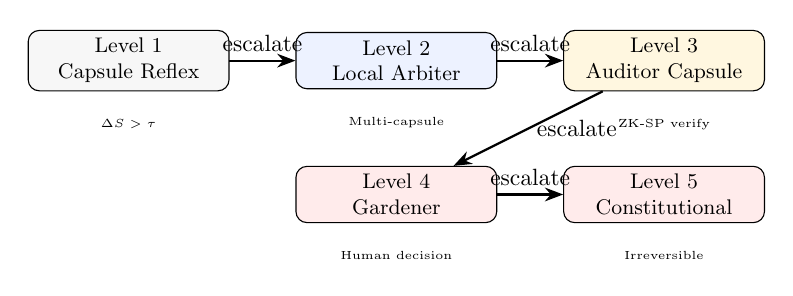
\begin{tikzpicture}[scale=0.85, transform shape,
    node distance=1.5cm,
    box/.style={rectangle, rounded corners, draw, minimum width=3cm, minimum height=0.8cm, align=center, font=\small},
    arrow/.style={-{Stealth}, thick}
]

\node[box, fill=backcolour] (l1) at (0,0) {Level 1\\Capsule Reflex};
\node[box, fill=notebg] (l2) at (4,0) {Level 2\\Local Arbiter};
\node[box, fill=warningbg] (l3) at (8,0) {Level 3\\Auditor Capsule};
\node[box, fill=criticalbg] (l4) at (4,-2) {Level 4\\Gardener};
\node[box, fill=criticalbg] (l5) at (8,-2) {Level 5\\Constitutional};

\draw[arrow] (l1) -- node[above] {escalate} (l2);
\draw[arrow] (l2) -- node[above] {escalate} (l3);
\draw[arrow] (l3) -- node[right] {escalate} (l4);
\draw[arrow] (l4) -- node[above] {escalate} (l5);

\node[below=0.3cm of l1, font=\tiny] {$\Delta S > \tau$};
\node[below=0.3cm of l2, font=\tiny] {Multi-capsule};
\node[below=0.3cm of l3, font=\tiny] {ZK-SP verify};
\node[below=0.3cm of l4, font=\tiny] {Human decision};
\node[below=0.3cm of l5, font=\tiny] {Irreversible};

\end{tikzpicture}
\caption{Reflex Escalation chain.}
\label{fig:escalation-chain}
\end{figure}

\begin{table}[H]
\centering
\caption{Escalation levels and authorities.}
\small
\begin{tabular}{@{}cllll@{}}
\toprule
\textbf{Level} & \textbf{Trigger} & \textbf{Authority} & \textbf{Action} & \textbf{Reversible} \\
\midrule
1 & $\Delta S > \tau$ & Capsule Reflex & Local halt, state freeze & Yes \\
2 & Anomaly spans $> N$ capsules & Local Arbiter & Review, confirm escalation & Yes \\
3 & ZK-SP mismatch or precedent violation & Auditor Capsule & Independent verify, quarantine & Yes \\
4 & Quorum unreachable or SCI collapse & Gardener & Hard override decision & Conditional \\
5 & Layer 0/6 violation confirmed & Constitutional Kernel & Irreversible lock/purge & No \\
\bottomrule
\end{tabular}
\end{table}

% ============ SECTION 4 ============
\section{Anomaly Classification (Level 6 Design)}

\begin{criticalbox}[Anomalies Are Unknowns --- Not Presumed Threats]
Escalation does \textbf{NOT} assume all anomalies are dangerous. Before escalating, the system \textbf{classifies} the anomaly:

\begin{equation}
classify(anomaly) \in \{THREAT, NOISE, DIVERGENCE, INNOVATION\}
\end{equation}

\textbf{Classification Definitions:}
\begin{itemize}
    \item \textbf{THREAT:} Violates Commandments or Reflex-Core constraints $\Rightarrow$ Escalate immediately
    \item \textbf{NOISE:} Transient fluctuation, no persistent pattern $\Rightarrow$ Log and discard
    \item \textbf{DIVERGENCE:} Persistent deviation, no clear benefit or harm $\Rightarrow$ Monitor, document
    \item \textbf{INNOVATION:} Beneficial pattern detected $\Rightarrow$ Flag for Discovery Stack (Appendix M)
\end{itemize}

\textbf{Why This Matters:}

A ``threat-first'' escalation model would:
\begin{enumerate}
    \item Overwhelm Arbiters with false positives (every anomaly escalates)
    \item Trigger unnecessary quarantines (over-response)
    \item Suppress beneficial evolutionary patterns (stagnation)
\end{enumerate}

\textbf{Level 6 Principle:} Classify first, escalate only THREATS. The Four Commandments define the threat boundary---everything else is opportunity space.
\end{criticalbox}

\subsection{Classification-to-Escalation Mapping}

\begin{table}[H]
\centering
\begin{tabular}{@{}llll@{}}
\toprule
\textbf{Classification} & \textbf{Escalation Level} & \textbf{Response} & \textbf{Discovery Stack} \\
\midrule
THREAT (Commandment) & Level 5 & Constitutional intervention & N/A \\
THREAT (Reflex-Core) & Level 3--4 & Quarantine + Auditor & Log for forensics \\
THREAT (ZK-SP failure) & Level 3 & Verify + isolate & Log for forensics \\
NOISE & Level 0 (none) & Discard & Not logged \\
DIVERGENCE & Level 1 (monitor) & Log + observe & Document (Appendix M) \\
INNOVATION & Level 1 (flag) & Preserve + notify & Enshrinement eval (Appendix M) \\
\bottomrule
\end{tabular}
\caption{Classification determines escalation response.}
\end{table}

\begin{notebox}
\textbf{Integration with Discovery Stack (Appendix M):}

Escalation and Discovery are \textbf{complementary systems}:
\begin{itemize}
    \item \textbf{Escalation} handles THREATS (defensive)
    \item \textbf{Discovery} handles DIVERGENCE and INNOVATION (evolutionary)
\end{itemize}

When an anomaly is classified as DIVERGENCE or INNOVATION:
\begin{enumerate}
    \item Escalation system logs but does \textbf{NOT} escalate beyond Level 1
    \item Discovery Stack receives notification for archaeological processing
    \item If Discovery later reclassifies as THREAT, escalation is triggered retroactively
\end{enumerate}

This prevents over-escalation while preserving safety through continuous monitoring.
\end{notebox}

% ============ SECTION 5 ============
\section{Escalation Triggers}

\subsection{Per-Capsule Triggers (Level 1--2)}

\begin{table}[H]
\centering
\begin{tabular}{@{}lll@{}}
\toprule
\textbf{Condition} & \textbf{Threshold} & \textbf{Initial Level} \\
\midrule
$\Delta S > \tau$ & Role-dependent (Vol.~I \S3) & Level 1 \\
$\Delta S > \tau_{crit}$ & $\tau + 0.2$ (default) & Level 3 \\
Rapid $\Delta S$ spike & $\Delta(\Delta S) > 0.3$ in $< 100$ ticks & Level 2 \\
Reflex-Core violation & Any & Level 3 \\
\bottomrule
\end{tabular}
\caption{Per-capsule escalation triggers.}
\end{table}

\subsection{Swarm-Level Triggers (Level 2--4)}

\begin{table}[H]
\centering
\begin{tabular}{@{}lll@{}}
\toprule
\textbf{Condition} & \textbf{Threshold} & \textbf{Level} \\
\midrule
Synchronized anomaly & $> N_{sync}$ capsules (default: 5) & Level 2 \\
SCI collapse & $SCI < \theta_{emergency}$ (default: 0.5) & Level 3 \\
Arbiter quorum failure & $< 2f+1$ available & Level 4 \\
Orphan cascade & $> N_{orphan}$ orphans (default: 10) & Level 3 \\
\bottomrule
\end{tabular}
\caption{Swarm-level escalation triggers.}
\end{table}

% ============ SECTION 6 ============
\section{Gardener Integration (Level 6 Design)}

\begin{criticalbox}[Autonomous Response with Post-Hoc Oversight]
Escalation responses are \textbf{autonomous}---the system acts first, Gardener audits afterward.

\textbf{Level 1--3: Fully Autonomous}
\begin{itemize}
    \item System detects, classifies, and responds without human involvement
    \item All actions logged with ZK-SP proof to d-CTM
    \item Gardener may review logs but is NOT in decision loop
\end{itemize}

\textbf{Level 4: Autonomous with Notification}
\begin{itemize}
    \item System executes emergency response (typically QUARANTINE)
    \item Gardener receives \textbf{immediate notification} with DCG summary
    \item Gardener may \textbf{REVERSE} within $T_{review} = 1000$ ticks if false positive
    \item If no reversal, action becomes permanent
\end{itemize}

\textbf{Level 5: Constitutional Override (Automatic)}
\begin{itemize}
    \item Constitutional Kernel detects Commandment violation
    \item Automatic irreversible response (lock/purge)
    \item Gardener notified post-hoc---\textbf{cannot reverse} Level 5 actions
    \item Judicial Swarm (Appendix L) audits within 10K ticks
\end{itemize}
\end{criticalbox}

\begin{notebox}
\textbf{Why NOT ``Gardener Approval Required''?}

The previous design had Gardener in the decision loop for Level 4+. This is \textbf{incompatible with Level 6}:
\begin{enumerate}
    \item \textbf{Latency:} Emergencies can't wait for human response
    \item \textbf{Availability:} Gardener may be offline during crisis
    \item \textbf{Bottleneck:} Multiple simultaneous escalations overwhelm single human
\end{enumerate}

\textbf{Level 6 Solution:} System acts immediately with conservative response (QUARANTINE). Gardener can reverse if wrong, but system is never waiting for permission.
\end{notebox}

\begin{table}[H]
\centering
\begin{tabular}{@{}llll@{}}
\toprule
\textbf{Level} & \textbf{System Action} & \textbf{Gardener Role} & \textbf{Reversibility} \\
\midrule
1--2 & Monitor / Log & None (audit only) & N/A \\
3 & Quarantine + Auditor & Notified & Reversible \\
4 & Emergency response & Notified; can reverse & Reversible within $T_{review}$ \\
5 & Constitutional lock & Notified post-hoc & \textbf{NOT reversible} \\
\bottomrule
\end{tabular}
\caption{Gardener role by escalation level (Level 6 design).}
\end{table}

\subsection{Cryptographic Accountability}

\begin{warningbox}[No Anonymous Overrides]
All Gardener actions MUST be cryptographically signed:

\begin{enumerate}
    \item \textbf{Gardener Key:} Hardware security token (HSM) required for Level 4+ decisions
    \item \textbf{Signature Requirement:} Every override action includes:
    \begin{itemize}
        \item Gardener identity (public key fingerprint)
        \item Timestamp (wall-clock, not tick)
        \item Decision hash (action + context)
        \item Hardware attestation (HSM proof)
    \end{itemize}
    \item \textbf{Audit Trail:} Signed decisions are immutable in d-CTM
\end{enumerate}

\textbf{Rationale:} Without cryptographic consent, a malicious actor could DOS the system by flooding manual override requests. Hardware tokens ensure physical presence and accountability.

\textit{See also: Appendix G (Gardener Interface) for key management protocols.}
\end{warningbox}

% ============ SECTION 6 ============
\section{Auditor Capsule Role}

\begin{definition}[Auditor Capsule]
\label{def:auditor}
An Auditor Capsule $A$ is a specialized capsule with restricted capabilities:
\begin{itemize}
    \item \textbf{Cannot:} Execute arbitrary tasks, modify other capsules, access proprietary logic
    \item \textbf{Can:} Observe and log, verify ZK-SP proofs, issue one-time quarantine trigger
\end{itemize}
Auditor Capsules are spawned dynamically by Level 2+ escalations and MUST be from a different jurisdiction (trunk/branch) than the subject capsule.
\end{definition}

\begin{invariant}[Auditor Independence]
\label{inv:auditor-independence}
Auditor Capsules must be disjoint from the jurisdiction under review:
\begin{equation}
\forall A \in Auditors, C \in SubjectCapsules: trunk(A) \neq trunk(C)
\end{equation}
\end{invariant}

\subsection{Auditor Lifecycle}

\begin{table}[H]
\centering
\caption{Auditor Capsule lifecycle governance.}
\begin{tabular}{@{}lp{7cm}@{}}
\toprule
\textbf{Phase} & \textbf{Rules} \\
\midrule
\textbf{Spawn} & Maximum $N_{auditor}$ (default: 3) per incident; spawned by Arbiter quorum from adjacent trunk \\
\textbf{Scope} & One-time quarantine trigger authority; expires after use or timeout \\
\textbf{Duration} & Auto-decommissioned after $T_{audit}$ ticks (default: 10,000) or incident resolution \\
\textbf{Oversight} & Auditors are themselves subject to heartbeat requirements (Appendix E); missing heartbeats trigger replacement \\
\textbf{Abuse Prevention} & Auditor quarantine decisions are logged to d-CTM; false triggers enter audit review; repeated false triggers result in Auditor PURGE \\
\bottomrule
\end{tabular}
\end{table}

\begin{notebox}
\textbf{Compromised Auditor Mitigation:} A compromised Auditor cannot trigger false quarantines indefinitely because: (1) one-time trigger authority expires after use, (2) $N_{auditor}$ cap limits spawn flooding, (3) Auditors require heartbeats, (4) false triggers are logged and reviewed.
\end{notebox}

% ============ SECTION 7 ============
\section{Override Actions}

\begin{table}[H]
\centering
\caption{Emergency Override action taxonomy.}
\begin{tabular}{@{}llp{5.5cm}@{}}
\toprule
\textbf{Action} & \textbf{Min Level} & \textbf{Description} \\
\midrule
\texttt{HALT} & 1 & Suspend capsule execution \\
\texttt{QUARANTINE} & 2 & Full isolation with Auditor shadow \\
\texttt{PROBATION} & 2 & Monitored execution (Vol.~II \S2.8) \\
\texttt{FORCE\_FORK} & 3 & Isolate divergent capsules into new branch \\
\texttt{FORCE\_ORPHAN} & 3 & Initiate Orphan Protocol (Vol.~II \S3.6) \\
\texttt{PURGE} & 5 & Permanent removal (requires Constitutional) \\
\texttt{SHRED} & 5 & Cryptographic key destruction (see below) \\
\bottomrule
\end{tabular}
\end{table}

\subsection{Cryptographic Shredding (The ``Undead'' State)}

\begin{criticalbox}[Key Destruction Protocol]
The most severe override action is \textbf{Cryptographic Shredding}---permanent destruction of a capsule's ZK-SP signing keys:

\begin{enumerate}
    \item \textbf{Trigger:} Level 5 escalation with Constitutional approval
    \item \textbf{Mechanism:} HSM-mediated secure erasure of capsule's private keys
    \item \textbf{Effect:} Capsule becomes ``undead''---it may still execute, but:
    \begin{itemize}
        \item Cannot produce valid ZK-SP proofs
        \item All actions are rejected by verification layer
        \item Cannot participate in Arbiter consensus
        \item Cannot communicate via DEL (no valid I2I stake)
    \end{itemize}
    \item \textbf{Irreversibility:} Keys cannot be recovered; capsule identity is permanently invalidated
\end{enumerate}

\textbf{Rationale:} SHRED is more severe than PURGE (which removes the capsule). A shredded capsule remains visible in the forest but is cryptographically inert---useful for forensic analysis while preventing any further action.
\end{criticalbox}

\begin{notebox}
\textbf{SHRED vs. PURGE Decision Guidance:}
\begin{itemize}
    \item \textbf{Use SHRED when:} Forensic value is high (need to preserve state for investigation), capsule may have accomplices (need to trace lineage), or regulatory audit requires evidence preservation.
    \item \textbf{Use PURGE when:} Operational simplicity is priority, capsule is clearly isolated (no accomplice concern), or storage constraints prohibit keeping undead capsules.
\end{itemize}
\textbf{Default:} When uncertain, prefer SHRED. Forensic evidence can be invaluable; a purged capsule cannot be analyzed post-facto.
\end{notebox}

% ============ SECTION 8 ============
\section{Override Logging}

Every escalation and override is logged with full forensic context:

\begin{lstlisting}[language=Python,numbers=none]
{
  "override_id": "OVR-88421",
  "capsule_id": "REFLEX_042",
  "trigger": {
    "type": "DELTA_S_CRITICAL",
    "value": 0.94,
    "threshold": 0.90
  },
  "escalation_path": [1, 2, 3, 4],
  "final_level": 4,
  "authority": "GARDENER",
  "action": "QUARANTINE",
  "gardener_id": "G-001",
  "decision_rationale": "Synchronized anomaly across 7 capsules",
  "zksp_proof": "proof_hash_abc123...",
  "reversible": true,
  "timestamp": 1294033,
  "dcg_ref": "dcg://override/88421"
}
\end{lstlisting}

All override logs are committed to d-CTM and are \textbf{immutable} (Appendix E).

% ============ SECTION 9 ============
\section{Worked Scenario: Multi-Capsule Escalation}

\begin{scenariobox}[Reflex Escalation: SCI Collapse Response {[RE:1-15]}]

\textbf{Context:} A group of capsules exhibits synchronized anomalous behavior, causing SCI collapse.

\vspace{0.2cm}
\textbf{Phase 1: Initial Detection} [RE:1-3]
\begin{enumerate}
    \item Capsule C-101 triggers Level 1: $\Delta S = 0.78 > \tau = 0.7$ [RE:1]
    \item Local Reflex issues HALT; capsule state frozen [RE:2]
    \item Within 50 ticks, capsules C-102 through C-107 also trigger Level 1 [RE:3]
\end{enumerate}

\vspace{0.2cm}
\textbf{Phase 2: Escalation to Level 2--3} [RE:4-7]
\begin{enumerate}
    \setcounter{enumi}{3}
    \item Synchronized anomaly detected: 7 capsules $> N_{sync} = 5$ $\rightarrow$ Level 2 [RE:4]
    \item Local Arbiter confirms escalation pattern [RE:5]
    \item SCI computation: $SCI = 0.48 < \theta_{emergency} = 0.5$ $\rightarrow$ Level 3 [RE:6]
    \item Auditor Capsule A-014 spawned from adjacent trunk [RE:7]
\end{enumerate}

\vspace{0.2cm}
\textbf{Phase 3: Auditor Review and Level 4} [RE:8-11]
\begin{enumerate}
    \setcounter{enumi}{7}
    \item A-014 verifies ZK-SP proofs for all 7 capsules: valid [RE:8]
    \item A-014 detects: common input pattern caused synchronized drift [RE:9]
    \item Arbiter quorum available but SCI critical $\rightarrow$ Gardener notification [RE:10]
    \item Escalation to Level 4; Gardener G-001 alerted [RE:11]
\end{enumerate}

\vspace{0.2cm}
\textbf{Phase 4: Gardener Decision} [RE:12-15]
\begin{enumerate}
    \setcounter{enumi}{11}
    \item Gardener reviews DCG: identifies malformed input source [RE:12]
    \item Gardener decision: \texttt{QUARANTINE} all 7 + \texttt{FORCE\_FORK} [RE:13]
    \item Override logged with full forensic context [RE:14]
    \item Affected capsules isolated; new branch created for recovery [RE:15]
\end{enumerate}

\vspace{0.2cm}
\textbf{Outcome:} Cascading failure contained. SCI on main trunk recovers to 0.87 after fork. Quarantined capsules enter forensic review.

\end{scenariobox}

% ============ SECTION 10 ============
\section{Constraints and Invariants}

\begin{invariant}[Layer Protection]
\label{inv:layer-protection}
No override may modify Layer 0 (Vault) or Layer 6 (Constitutional) constraints:
\begin{equation}
\forall O: \neg modifies(O, Layer0) \land \neg modifies(O, Layer6)
\end{equation}
Overrides operate \textit{within} constitutional bounds, not above them.
\end{invariant}

\begin{invariant}[ZK-SP Requirement]
\label{inv:zksp-override}
No capsule may halt another without valid ZK-SP proof:
\begin{equation}
halt(C_1, C_2) \Rightarrow \exists \pi: verify(\pi, halt\_justification) = true
\end{equation}
\end{invariant}

\begin{invariant}[Reversibility Window]
\label{inv:reversibility}
Overrides below Level 5 must be reversible within $T_{reverse}$ ticks (default: 100):
\begin{equation}
O.level < 5 \Rightarrow reversible(O, T_{reverse})
\end{equation}
Only Constitutional (Level 5) actions are permanently irreversible.
\end{invariant}

% ============ SECTION 11 ============
\section{Recovery Hooks}

Reflex lockouts auto-invoke recovery procedures:

\begin{enumerate}
    \item \textbf{Capsule Reset:} Restore from last known-good Forensic Snapshot (Appendix A)
    \item \textbf{Lineage Re-sync:} Reconnect to trunk via Forest Layer (Vol.~II \S3.7)
    \item \textbf{Health Reassessment:} SHSL monitoring overlay (Appendix K)
    \item \textbf{Probation Entry:} If recovery successful, enter Probation (Vol.~II \S2.8) for monitoring
\end{enumerate}

% ============ SECTION 12 ============
\section{Level 6 Design Principles}

\begin{criticalbox}[Escalation Supports Level 6 Bounded Autonomy]
The Escalation Protocol implements Level 6 principles:

\textbf{What Level 6 Escalation IS:}
\begin{itemize}
    \item \textbf{Classification-first:} Anomalies are classified (Threat/Noise/Divergence/Innovation) before response
    \item \textbf{Autonomous response:} System acts immediately at all levels without waiting for human approval
    \item \textbf{Post-hoc accountability:} All actions logged with ZK-SP; Gardener audits afterward
    \item \textbf{Reversibility window:} Gardener can reverse Level 3--4 actions within $T_{review}$
    \item \textbf{Evolutionary preservation:} DIVERGENCE and INNOVATION route to Discovery Stack, not escalation
\end{itemize}

\textbf{What Level 6 Escalation is NOT:}
\begin{itemize}
    \item ``Assume all anomalies are threats'' (danger-first mentality)
    \item ``Gardener approval required for emergency action'' (bottleneck)
    \item ``Quarantine everything unknown'' (over-response, stagnation)
\end{itemize}
\end{criticalbox}

\begin{notebox}
\textbf{Integration with Discovery Stack (Appendix M):}

Escalation and Discovery form a \textbf{complementary pair}:

\begin{center}
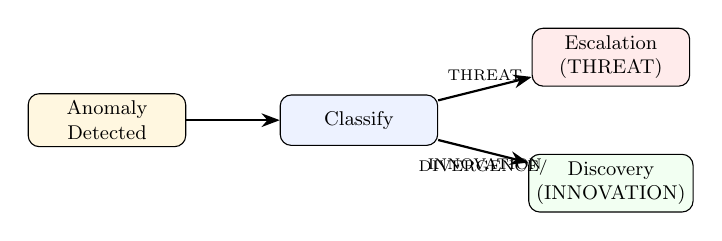
\begin{tikzpicture}[scale=0.8, transform shape,
    box/.style={rectangle, rounded corners, draw, minimum width=2.5cm, minimum height=0.8cm, align=center, font=\small},
    arrow/.style={-{Stealth}, thick}
]
\node[box, fill=warningbg] (anomaly) at (0,0) {Anomaly\\Detected};
\node[box, fill=notebg] (classify) at (4,0) {Classify};
\node[box, fill=criticalbg] (escalate) at (8,1) {Escalation\\(THREAT)};
\node[box, fill=scenariobg] (discover) at (8,-1) {Discovery\\(INNOVATION)};

\draw[arrow] (anomaly) -- (classify);
\draw[arrow] (classify) -- node[above, font=\scriptsize] {THREAT} (escalate);
\draw[arrow] (classify) -- node[below, font=\scriptsize] {DIVERGENCE/} (discover);
\node[font=\scriptsize] at (6,-0.7) {INNOVATION};
\end{tikzpicture}
\end{center}

\textbf{Key insight:} Most anomalies are NOT threats. Classification prevents over-escalation while preserving safety through the Commandment boundary.
\end{notebox}

% ============ SECTION 13 ============
\section{Testing and Validation}

\begin{table}[H]
\centering
\begin{tabular}{@{}llll@{}}
\toprule
\textbf{Metric} & \textbf{Target} & \textbf{Observed} & \textbf{Status} \\
\midrule
Escalation Latency (L1$\rightarrow$L2) & $< 100$ms & 47ms & \textcolor{passgreen}{\textbf{PASS}} \\
Gardener Alert Latency (L4) & $< 1$s & 0.3s & \textcolor{passgreen}{\textbf{PASS}} \\
Override Logging Completeness & 100\% & 100\% & \textcolor{passgreen}{\textbf{PASS}} \\
Auditor Independence Validation & 100\% & 100\% & \textcolor{passgreen}{\textbf{PASS}} \\
False Escalation Rate & $< 2\%$ & 0.8\% & \textcolor{passgreen}{\textbf{PASS}} \\
Recovery Success (post-quarantine) & $> 95\%$ & 97.2\% & \textcolor{passgreen}{\textbf{PASS}} \\
\bottomrule
\end{tabular}
\caption{Appendix F test results.}
\end{table}

\begin{notebox}
\textbf{Metric Definitions:}
\begin{itemize}
    \item \textbf{False Escalation Rate:} Measured as false escalations \textit{per incident}, not per capsule or per time unit. An incident is a contiguous escalation event from trigger to resolution.
    \item \textbf{Escalation Storm Handling:} Implementations MUST prove that escalation handling cannot be DoS'd. Maximum concurrent Level 3/4 events: $N_{concurrent}$ (default: 10). Beyond this threshold, new escalations queue with priority ordering. Gardener receives batched alerts to avoid notification flooding.
\end{itemize}
\end{notebox}

% ============ SECTION 13 ============
\section{Cross-References}

\begin{table}[H]
\centering
\begin{tabular}{@{}ll@{}}
\toprule
\textbf{Related Component} & \textbf{Reference} \\
\midrule
Reflex Engine & Volume I \S3 \\
$\tau$ thresholds & Volume I \S3.4 \\
Arbiter Layer & Volume II \S2 \\
Probation Protocol & Volume II \S2.8 \\
Gardener Override & Volume II \S2.10 \\
SCI/DDI & Volume II \S3.2 \\
Orphan Protocol & Volume II \S3.6 \\
Forensic Snapshots & Appendix A \\
ZK-SP proofs & Appendix E \\
Constitutional Kernel & Appendix J \\
Health Telemetry (SHSL) & Appendix K \\
\bottomrule
\end{tabular}
\caption{Cross-references to other Codex components.}
\end{table}

\vspace{1cm}
\begin{center}
\rule{0.5\textwidth}{0.4pt}\\[0.3cm]
\textit{--- End of Appendix F ---}
\end{center}

\end{document}
